\documentclass[tikz,preview]{standalone}
\usepackage{standalone}
\usepackage[version=4]{mhchem}
\definecolor{skyblue}{RGB}{0, 255, 255}
\begin{document}
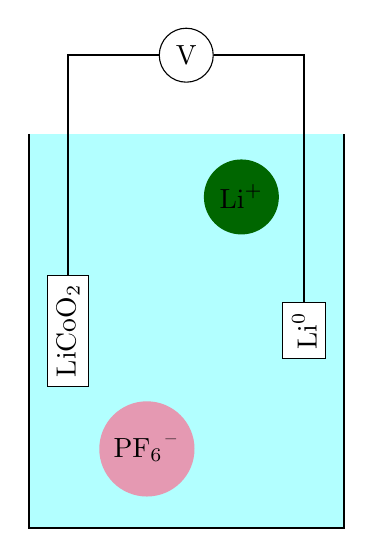
\begin{tikzpicture}
  \draw[fill=skyblue!30, draw=none] (0,0) ++(-2,-2.5) -| ++(4,5) -| cycle {};
  \draw[thick] (0,0) ++(-2,2.5) |- ++(4,-5) -- ++(0,5);
  \node[circle,draw=black] (V) at (0,3.5) {V};
  \node[rectangle,draw=black,rotate=90,fill=white] (n) at (1.5,0) {\ce{Li^0}};
  \node[rectangle,draw=black,rotate=90,fill=white] (p) at (-1.5,0) {\ce{LiCoO2}};
  \node[circle,draw=none,fill=purple!40] (pf6) at (-0.5,-1.5) {\ce{PF6^-}};
  \node[circle,draw=none,fill=green!40!black] (li) at (0.7,1.7) {\ce{Li^+}};
  % lines
  \draw[thick] (p.east) |- (V.west);
  \draw[thick] (n.east) |- (V.east);
\end{tikzpicture}
\end{document}